\documentclass[11pt,a4paper,French]{article}
\usepackage{subfiles}
\usepackage{float}
\usepackage{fancyhdr}
\pagestyle{fancy}
\fancyhf{}
\usepackage{hyperref}
\usepackage{tcolorbox}
\tcbuselibrary{theorems}
\usepackage[utf8]{inputenc}
\usepackage[T1]{fontenc}
\usepackage{pifont}
\usepackage[french]{babel}
%%Mon clavier est en qwerty, pas d'accent donc pour moi
\newcommand{\e}{\'{e}}
\newcommand{\h}{Hoare}
\usepackage{listings}
\usepackage{amsfonts}
\usepackage{graphicx}
\usepackage{tikz}
\usetikzlibrary{fadings}
\usetikzlibrary{trees}
%%Header
%TODO
  %\usepackage{fancyhdr}
  %\pagestyle{fancy}
%%
\usepackage{xcolor}
\newtheorem{definition}{Definition}[section]
\usepackage{titlesec}
\usepackage{pagecolor,lipsum}
%%Nordic color
  \definecolor{Nblack}{HTML}{3b4252}
  \definecolor{NBLACK}{HTML}{2e3440}
  \definecolor{Nwhite}{HTML}{eceff4}
  \definecolor{nwhite}{HTML}{e5e9f0}
  \definecolor{Nblue}{HTML}{5e81ac}
  \definecolor{Nred}{HTML}{bf616a}
  \definecolor{nred}{HTML}{d08770}
  \definecolor{Nurl}{HTML}{8fbcbb}
  \definecolor{nblue}{HTML}{81a1c1}
  \let\oldtextbf\textbf
  \renewcommand{\textbf}[1]{\textcolor{NBLACK}{\oldtextbf{#1}}}
  \makeatletter
  \newcommand{\globalcolor}[1]{%
    \color{#1}\global\let\default@color\current@color
  }
  \makeatother
  \AtBeginDocument{\globalcolor{Nblack}}
  \titleformat{\section}
  {\color{Nblue}\normalfont\Large\bfseries}
  {\color{Nblue}\thesection}{1em}{}
  \titleformat{\subsection}
  {\color{nblue}\normalfont\large\bfseries}
  {\color{nblue}\thesubsection}{1em}{}
  \hypersetup{
      colorlinks=true,
      linkcolor=nblue,
      filecolor=magenta,      
      urlcolor=cyan,
      pdftitle={Overleaf Example},
      pdfpagemode=FullScreen,
      }
\lstdefinestyle{C}{
    backgroundcolor=\color{nwhite},   
    commentstyle=\color{green},
    keywordstyle=\color{nred},
    frame=single
    numberstyle=\tiny\color{gray},
    stringstyle=\color{purple},
    basicstyle=\footnotesize,
    breakatwhitespace=false,         
    breaklines=true,                 
    captionpos=b,                    
    keepspaces=true,                 
    showspaces=false,                
    showstringspaces=false,
    showtabs=false,                  
    tabsize=2,
    language=C
}
\rhead{\color{nblue}Hoare}
\lhead{\color{nblue}Rendue \LaTeX}
\rfoot{Page \thepage}
\newtcbtheorem[number within=section]{mytheo}{Propri\e t\e}%
{colback=Nblue!5,colframe=Nblue!35!NBLACK,fonttitle=\bfseries}{th}
%%
\begin{document}
\pagecolor{Nwhite}
\begin{titlepage}
%Title Page of Hoar
\begin{center}
  \vspace*{1cm}
  \Huge \textbf{Tony Hoare}

  \Large{Un bref apercue}

  \large{Par Th\e o.H }
  \vspace{0.8cm}

   \begin{minipage}{0.6\textwidth}
    \large \em{\hspace*{20mm}\flq{}There are two methods in

    software design. One is to make the program so simple,

     there are obviously no errors.}

    {The other is to make it so complicated,

    there are no obvious errors.\frq{}}
  \end{minipage}
  \begin{minipage}{0.3\textwidth}
    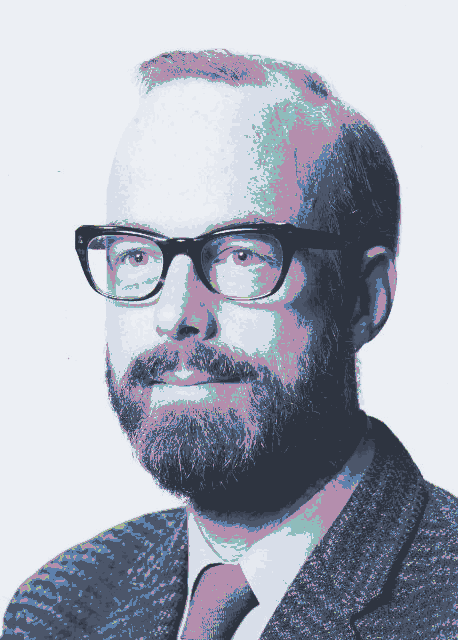
\includegraphics[width=\textwidth]{./img/PHoar.png}
  \end{minipage}
  \noindent
  \vfill
  \makebox[0pt][l]{\rule{1.3\textwidth}{1pt}}
{\huge \color{Nblue}{Édition scientifique avec \LaTeX}}
\vskip\baselineskip
\noindent
\color{nblue}\today
\end{center}
\end{titlepage}
%End title Page of Hoar

  \tableofcontents
  \subfile{Intro}
  \subfile{logique}
  \subfile{quicksort}
  \bibliography{lesson7a1} 
  \bibliographystyle{ieeetr}

\end{document}
